\section{Ice Thickness Evolution}
The evolution of the ice thickness, $H$, stems from the continuity equation and can be expressed as
\begin{equation}
  \label{kin.eq.ice_thickness}
  \frac{\pd H}{\pd t} = -\vec\nabla\cdot(\overline{\vec{u}} H) + B,
\end{equation}
where $\overline{\vec{u}}$ is the vertically averaged ice velocity, $B$ is the surface mass balance and $\vec\nabla$ is the horizontal gradient operator. 

For large--scale ice sheet models, the \emph{shallow ice approximation} is generally used. This approximation states that bedrock and ice surface slopes are assumed sufficiently small so that the normal stress components can be neglected. The horizontal shear stresses ($\tau_{xz}$ and $\tau_{yz}$) can thus be approximated by
\begin{equation}
  \label{kin.eq.horiz_shear}
  \begin{split}
    \tau_{xz}(z)&=-\rho g(s-z)\frac{\pd s}{\pd x},\\
    \tau_{yz}(z)&=-\rho g(s-z)\frac{\pd s}{\pd y},
  \end{split}
\end{equation}
where $\rho$ is the density of ice, $g$ the acceleration due to gravity and $s=H+h$ the ice surface.

Strain rates $\dot{\epsilon}_{ij}$ of polycrystalline ice are related to the stress tensor by the non--linear flow law:
\begin{equation}
  \label{kin.eq.flowlaw}
  \dot{\epsilon}_{iz}=\frac12\left(\frac{\pd u_i}{\pd z}+\frac{\pd u_z}{\pd i}\right)=A(T^\ast)\tau_\ast^{(n-1)}\tau_{iz}\qquad i=x,y,
\end{equation}
where $\tau_\ast$ is the effective shear stress defined by the second invariant of the stress tensor, $n$ the flow law exponent and $A$ the temperature--dependent flow law coefficient. $T^\ast$ is the absolute temperature corrected for the dependence of the melting point on pressure. The parameters $A$ and $n$ have to
 be found by experiment. $n$ is usually taken to be 3. $A$ depends on factors such as temperature, crystal size and orientation, and ice impurities. Experiments suggest that $A$ follows the Arrhenius relationship:
\begin{equation}
  \label{kin.eq.arrhenius}
  A(T^\ast)=fae^{-Q/RT^\ast},
\end{equation}where $a$ is a temperature--independent material constant, $Q$ is the activation energy for creep and $R$ is the universal gas constant. $f$ is a tuning parameter used to `speed--up' ice flow and accounts for ice impurities and the development of anisotropic ice fabrics.

Integrating \eqref{kin.eq.arrhenius} with respect to $z$ gives the horizontal velocity profile:
\begin{equation}
  \label{kin.eq.horiz_velo}
  \vec u(z)-\vec u(h) = -2(\rho g)^n|\vec\nabla s|^{n-1}\vec\nabla s\int_h^zA(s-z)^ndz,
\end{equation}
where $\vec u(h)$ is the basal velocity (sliding velocity). Integrating \eqref{kin.eq.horiz_velo} again with respect to $z$ gives an expression for the vertically averaged ice velocity:
\begin{equation}
  \label{kin.eq.avg_velo}
  \overline{\vec u}H=-2(\rho g)^n|\vec\nabla s|^{n-1}\vec\nabla s\int_h^s\int_h^zA(s-z)^ndzdz'.
\end{equation}

The vertical ice velocity stems from the conservation of mass for an incompressible material:
\begin{equation}
  \label{kin.eq.incompress}
  \frac{\pd u_x}{\pd x} + \frac{\pd u_y}{\pd y} + \frac{\pd u_z}{\pd z} = 0.
\end{equation}
Integrating \eqref{kin.eq.incompress} with respect to $z$ gives the vertical velocity distribution of each ice column:
\begin{equation}
  \label{kin.eq.vert_velo}
  w(z)=-\int_h^z\vec\nabla\cdot\vec u(z)dz+w(h),
\end{equation}
with lower, kinematic boundary condition
\begin{equation}
  w(h)=\frac{\pd h}{\pd t}+\vec u(h)\cdot\vec\nabla h+S,
\end{equation}
where $S$ is the melt rate at the ice base given by Equation \eqref{temp.eq.meltrate}. The upper kinematic boundary is given by the surface mass balance and must satisfy:
\begin{equation}
  \label{kin.eq.upper_bc}
  w(s)=\frac{\pd s}{\pd t}+\vec u(s)\cdot\vec\nabla s+B.
\end{equation}

\subsection{Numerical Grid}\label{num.sec.grid}
The continuous equations descrining ice physics have to be discretised in order to be solved by a computer (which is inherently finite). This section describes the finite--difference grids employed by the model.
\subsubsection{Horizontal Grid}
The modelled region ($x\in[0,L_x]$, $y\in[0,L_y]$) is discretised using a regular grid so that $x_i=(i-1)\Delta x$ for $i\in[1,N]$ (and similarly for $y_j$). The model uses two staggered horizontal grids in order to improve stability. Both grids use the same grid spacing, $\Delta x$ and $\Delta y$, but are off-set by half a grid (see Fig. \ref{kin.fig.grid}). 
\begin{figure}[htbp]
  \begin{center}
    \includegraphics{\dir/figs/grid.eps}
    \caption{Horizontal Grid.}
    \label{kin.fig.grid}
  \end{center}
\end{figure}
Quantities calculated on the $(r,s)$--grid are denoted with a tilde, i.e. $\tilde{F}$. Quantities are transformed between grids by averaging over the surrounding nodes, i.e. a quantity in the $(i,j)$--grid becomes in the $(r,s)$ grid:
\begin{subequations}
  \begin{align}
    \tilde{F}_{r,s}&=\tilde{F}_{i+\frac12,j+\frac12}=\frac14(F_{i,j}+F_{i+1,j}+F_{i+1,j+1}+F_{i,j+1})\\
    \intertext{and similarly for the reverse transformation:}
    F_{i,j}&=F_{r-\frac12,s-\frac12}=\frac14(\tilde{F}_{r-1,s-1}+\tilde{F}_{r,s-1}+\tilde{F}_{r,s}+\tilde{F}_{r-1,s})
  \end{align}
\end{subequations}

In general, horizontal velocities and associated quantities like the diffusivity are calculated on the $(r,s)$ grid, ice thickness, temperatures and vertical velocities are calculated on the $(i,j)$--grid.

Horizontal gradients are calculated on the $(r,s)$--grid, i.e. surface gradients are:
\begin{subequations}
\begin{align}
  \left(\frac{\pd s}{\pd x}\right)_{r,s}=\tilde{s}^x_{r,s}&=\frac{s_{i+1,j}-s_{i,j}+s_{i+1,j+1}-s_{i,j+1}}{2\Delta x}\\
  \left(\frac{\pd s}{\pd y}\right)_{r,s}=\tilde{s}^y_{r,s}&=\frac{s_{i,j+1}-s_{i,j}+s_{i+1,j+1}-s_{i+1,j}}{2\Delta y}
\end{align}  
\end{subequations}
Ice thickness gradients, $\tilde{H}^x_{r,s}$ and $\tilde{H}^y_{r,s}$, are formed similarly. Gradients in the $(r,s)$--grid are formed in a similar way, e.g. 
\begin{equation}
  \left(\frac{\pd u}{\pd x}\right)_{i,j}=u^x_{i,j}=\frac{\tilde{u}_{r,s-1}-\tilde{u}_{r-1,s-1}+\tilde{u}_{r,s}-\tilde{u}_{r-1,s}}{2\Delta x}
\end{equation}

\subsubsection{Periodic Boundary Conditions}
The model can be run with horizontal periodic boundary conditions, i.e. the western edge of the modelled region is joined with the eastern edge. Figure \ref{num.fig.grid_ew} illustrates the numeric grid when the model is run in torus mode.

\begin{figure}[htbp]
  \centering
  \includegraphics[width=0.9\textwidth]{\dir/figs/grid_ew.eps}
  \caption{A row of the numeric grid when the model is used in torus mode. Circles indicate points in $(i,j)$--grid and squares indicate points in the $(r,s)$--grid. Points with the same colour are logically the same.}
  \label{num.fig.grid_ew}
\end{figure}

These boundary conditions are enforced by exchanging points for the temperature and vertical velocity calculations. The ice thicknesses are calculated explicitly at the ghostpoints.

\subsubsection{$\sigma$--Coordinate System}\label{num.sec.sigma}
The vertical coordinate, $z$, is scaled by the ice thickness analogous to the $s$--coordinate in numerical weather simulations \citep[e.g.][]{Holton1992}. A new vertical coordinate, $\sigma$, is introduced so that the ice surface is at $\sigma=0$ and the ice base at $\sigma=1$ (see Fig. \ref{kin.fig.scale}), i.e.
\begin{equation}
  \label{kin.eq.vertical_scale}
  \sigma=\frac{s-z}{H}.
\end{equation}

\begin{figure}[htbp]
  \begin{center}
    \includegraphics{\dir/figs/scale.eps}
    \caption[Vertical scaling of the ice sheet model.]{Vertical scaling of the ice sheet model. The vertical axis is scaled to unity. The horizontal coordinates are not changed.}
    \label{kin.fig.scale}
  \end{center}
\end{figure}


The derivatives of a function $f$ in $(x,y,z,t)$ become in the new $(\tilde{x},\tilde{y},\sigma,\tilde{t})$ system:
\begin{subequations}
  \begin{align}
    \frac{\pd f}{\pd x} &= \frac{\pd f}{\pd\tilde{x}}+\frac1H\Delta_{\tilde{x}}\frac{\pd f}{\pd \sigma},\\
    \frac{\pd f}{\pd y} &= \frac{\pd f}{\pd\tilde{y}}+\frac1H\Delta_{\tilde{y}}\frac{\pd f}{\pd \sigma},\\
    \frac{\pd f}{\pd t} &= \frac{\pd f}{\pd\tilde{t}}+\frac1H\Delta_{\tilde{t}}\frac{\pd f}{\pd \sigma},\\
    \frac{\pd f}{\pd z} &= -\frac1H\frac{\pd f}{\pd\sigma},
  \end{align}
\end{subequations}
where  the geometric factors, $\Delta_{\tilde{x}}$, $\Delta_{\tilde{y}}$ and $\Delta_{\tilde{t}}$, are defined by
\begin{subequations}
  \begin{align}
  \Delta_{\tilde{x}}&=\left(\frac{\pd s}{\pd\tilde{x}}-\sigma\frac{\pd H}{\pd\tilde{x}}\right),\\
  \Delta_{\tilde{y}}&=\left(\frac{\pd s}{\pd\tilde{y}}-\sigma\frac{\pd H}{\pd\tilde{y}}\right),\\
  \Delta_{\tilde{t}}&=\left(\frac{\pd s}{\pd\tilde{t}}-\sigma\frac{\pd H}{\pd\tilde{t}}\right).
  \end{align}
\end{subequations}
The integral of $z$ becomes in the $\sigma$--coordinate system:
\begin{equation}
  \int_h^zfdz=-H\int_1^\sigma fd\sigma
\end{equation}

The vertical coordinate is discretised using an irregular grid spacing to reflect the fact that ice flow is more variable at the bottom of the ice column. In the vertical the index $k$ is used. 


\subsection{Ice Sheet Equations in $\sigma$--Coordinates}
The horizontal velocity, Equation \eqref{kin.eq.horiz_velo}, becomes in the $\sigma$--coordinate system
\begin{equation}
  \label{kin.eq.vert_velo_sigma}
  \vec u(\sigma) = -2(\rho g)^nH^{n+1}|\vec\nabla s|^{n-1}\vec\nabla s\int_1^\sigma A\sigma^nd\sigma+\vec u(1)
\end{equation}
and the vertically averaged velocity
\begin{equation}
  \label{kin.eq.avg_velo_scaled}
  \overline{\vec u} H=H\int_0^1\vec ud\sigma+\vec u(1)H
\end{equation}
The vertical velocity, Equation \eqref{kin.eq.vert_velo}, becomes
\begin{equation}
  \label{kin.eq.vert_velo_scaled}
  w(\sigma)=-\int_1^\sigma\left(\frac{\pd\vec u}{\pd\sigma}\cdot(\vec\nabla s-\sigma\vec\nabla H)+H\vec\nabla\cdot\vec u\right)d\sigma+w(1)
\end{equation}
and lower boundary condition
\begin{equation}
  w(1)=\frac{\pd h}{\pd t}+\vec u(1)\cdot\vec\nabla h+S.
\end{equation}

\subsection{Calculating the Horizontal Velocity and the Diffusivity}
Horizontal velocity and diffusivity calculations are split up into two parts:
\begin{subequations}
  \begin{align}
    \vec u(\sigma)&=c\vec\nabla s+\vec u(1)\\
    D &=H\int_0^1cd\sigma\\
    \vec q&=D\vec\nabla s+H\vec u(1)\\
    \intertext{with}
    c(\sigma)&=-2(\rho g)^nH^{n+1}|\vec\nabla s|^{n-1}\int_1^\sigma A\sigma^nd\sigma
  \end{align}
\end{subequations}

Quantities $\vec u$ and $D$ are found on the velocity grid. Integrating from the ice base ($k=N-1$), the discretised quantities become
\begin{subequations}
  \begin{equation}
    \tilde{c}_{r,s,N}=0
  \end{equation}
  \begin{multline}
    \tilde{c}_{r,s,k}=-2(\rho g)^nH_{r,s}^{n+1}\left(({\tilde{s}^x_{r,s}})^2+({\tilde{s}^y_{r,s}})^2\right)^{\frac{n-1}{2}}\\
    \sum_{\kappa=N-1}^k\frac{A_{r,s,\kappa}+A_{r,s,\kappa+1}}2 \left(\frac{\sigma_{\kappa+1}+\sigma_\kappa}2\right)^n(\sigma_{\kappa+1}-\sigma_\kappa)
  \end{multline}
  \begin{equation}
    \tilde{D}_{r,s}=H_{r,s}\sum_{k=0}^{N-1}\frac{\tilde{c}_{r,s,k}+\tilde{c}_{r,s,k+1}}2(\sigma_{k+1}-\sigma_k)
  \end{equation}
\end{subequations}
Expressions for $\vec{u}_{i,j,k}$ and $\vec{q}_{i,j}$ are straight forward.

\subsection{Solving the Ice Thickness Evolution Equation}
\subsubsection{Linearised Semi--Implicit Scheme}
Equation \eqref{kin.eq.ice_thickness} can be rewritten as a diffusion equation, with non--linear diffusion coefficient $D$:
\begin{equation}
  \label{kin.eq.ice_evo}
  \frac{\pd H}{\pd t}=-\vec\nabla\cdot D\vec\nabla s+B=\vec\nabla\cdot\vec q+B
\end{equation}
This non--linear partial differential equation can be linearised by using the diffusion coefficient from the previous time step. The diffusion coefficient is calculated on the $(r,s)$--grid, i.e. staggered in both $x$ and $y$ direction. Using finite differences, the fluxes in $x$ direction, $q^x$ become
\begin{subequations}
\begin{align}
  q^x_{i+\frac12,j}&=-\frac12(\tilde{D}_{r,s}+\tilde{D}_{r,s-1})\frac{s_{i+1,j}-s_{i,j}}{\Delta x}\\
  q^x_{i-\frac12,j}&=-\frac12(\tilde{D}_{r-1,s}+\tilde{D}_{r-1,s-1})\frac{s_{i,j}-s_{i-1,j}}{\Delta x}\\
  \intertext{and the fluxes in $y$ direction}
  q^y_{i,j+\frac12}&=-\frac12(\tilde{D}_{r,s}+\tilde{D}_{r-1,s})\frac{s_{i,j+1}-s_{i,j}}{\Delta y}\\
  q^y_{i,j-\frac12}&=-\frac12(\tilde{D}_{r,s-1}+\tilde{D}_{r-1,s-1})\frac{s_{i,j}-s_{i,j-1}}{\Delta y}
\end{align}  
\end{subequations}

Using the Crank--Nicolson scheme, the semi--implicit temporal discretisation of \eqref{kin.eq.ice_evo} is then:
\begin{multline}
\label{kin.eq.ice_evo_disc1}
  \frac{H^{t+1}_{i,j}-H^t_{i,j}}{\Delta t}=\frac{q^{x,t+1}_{i+\frac12,j}-q^{x,t+1}_{i-\frac12,j}}{2\Delta x}+\frac{q^{y,t+1}_{i,j+\frac12}-q^{y,t+1}_{i,j-\frac12}}{2\Delta y} \\
  +\frac{q^{x,t}_{i+\frac12,j}-q^{x,t}_{i-\frac12,j}}{2\Delta x}+\frac{q^{y,t}_{i,j+\frac12}-q^{y,t}_{i,j-\frac12}}{2\Delta y}+ B_{i,j}
\end{multline}
The superscripts $^t$ and $^{t+1}$ indicate at what time the ice thickness $H$ is evaluated. Collecting all $H^{t+1}$ terms of \eqref{kin.eq.ice_evo_disc1} on the LHS and moving all other terms to the RHS we can rewrite \eqref{kin.eq.ice_evo_disc1} as
\begin{equation}
  \label{kin.eq.evo_matrix}
  -\alpha_{i,j}H^{t+1}_{i-1,j} - \beta_{i,j}H^{t+1}_{i+1,j} - \gamma_{i,j}H^{t+1}_{i,j-1} - \delta_{i,j}H^{t+1}_{i,j+1}+ (1-\epsilon_{i,j})H^{t+1}_{i,j} = \zeta_{i,j}
\end{equation}
with the RHS,
\begin{multline}
  \zeta_{i,j} = \alpha_{i,j}H^{t}_{i-1,j} + \beta_{i,j}H^{t}_{i+1,j} + \gamma_{i,j}H^{t}_{i,j-1} + \delta_{i,j}H^{t}_{i,j+1} + (1+\epsilon_{i,j})H^{t}_{i,j} \\
  + 2(\alpha_{i,j}h_{i-1,j} + \beta_{i,j}h_{i+1,j} + \gamma_{i,j}h_{i,j-1} + \delta_{i,j}h_{i,j+1}+ \epsilon_{i,j}h_{i,j}) + B_{i,j}\Delta t
\end{multline}
with the elements of the sparse matrix
\begin{subequations}
  \begin{align}
    \alpha_{i,j} &=\frac{\tilde{D}_{r-1,s}+\tilde{D}_{r-1,s-1}}{4\Delta x^2}\Delta t\\
    \beta_{i,j} &=\frac{\tilde{D}_{r,s}+\tilde{D}_{r,s-1}}{4\Delta x^2}\Delta t\\
    \gamma_{i,j} &=\frac{\tilde{D}_{r,s-1}+\tilde{D}_{r-1,s-1}}{4\Delta y^2}\Delta t\\
    \delta_{i,j} &=\frac{\tilde{D}_{r,s}+\tilde{D}_{r-1,s}}{4\Delta y^2}\Delta t\\
    \epsilon_{i,j} &=-(\alpha_{i,j}+\beta_{i,j}+\gamma_{i,j}+\delta_{i,j})
  \end{align}
\end{subequations}

This matrix equation is solved using an iterative matrix solver for non-symmetric sparse matrices. The solver used here is the bi--conjugate gradient method with incomplete LU decomposition preconditioning provided by the SLAP package.

\subsubsection{Non--Linear Scheme}
The non--linearity of Equation \eqref{kin.eq.ice_evo} arises from the dependance of $D$ on $s$. A non--linear scheme for \eqref{kin.eq.ice_evo} can be formulated using Picard iteration, which consists of two iterations: an outer, non--linear and an inner, linear equation. The scheme is started off with the diffusivity from the previous time step, i.e.
\begin{subequations}
  \begin{equation}
    D^{(0),t+1}=D^{t}
  \end{equation}
and Equation \eqref{kin.eq.evo_matrix} becomes
\begin{multline}
  \label{kin.eq.evo_matrix_nonlin}
  -\alpha^{(\xi),t+1}_{i,j}H^{t+1}_{i-1,j} - \beta^{(\xi),t+1}_{i,j}H^{(\xi+1),t+1}_{i+1,j} - \gamma^{(\xi),t+1}_{i,j}H^{(\xi+1),t+1}_{i,j-1} \\
  - \delta^{(\xi),t+1}_{i,j}H^{(\xi+1),t+1}_{i,j+1}+ (1-\epsilon^{(\xi),t+1}_{i,j})H^{(\xi+1),t+1}_{i,j} = \zeta^{(0),t}_{i,j}
\end{multline}
\end{subequations}
Equation \eqref{kin.eq.evo_matrix_nonlin} is iterated over $\xi$ until the maximum ice thickness residual is smaller than some threshold:
\begin{equation}
  \max\left(\left|H^{(\xi+1),t+1}-H^{(\xi),t+1}\right|\right)<H_{\text{res}}
\end{equation}

\begin{figure}[htbp]
  \centering
  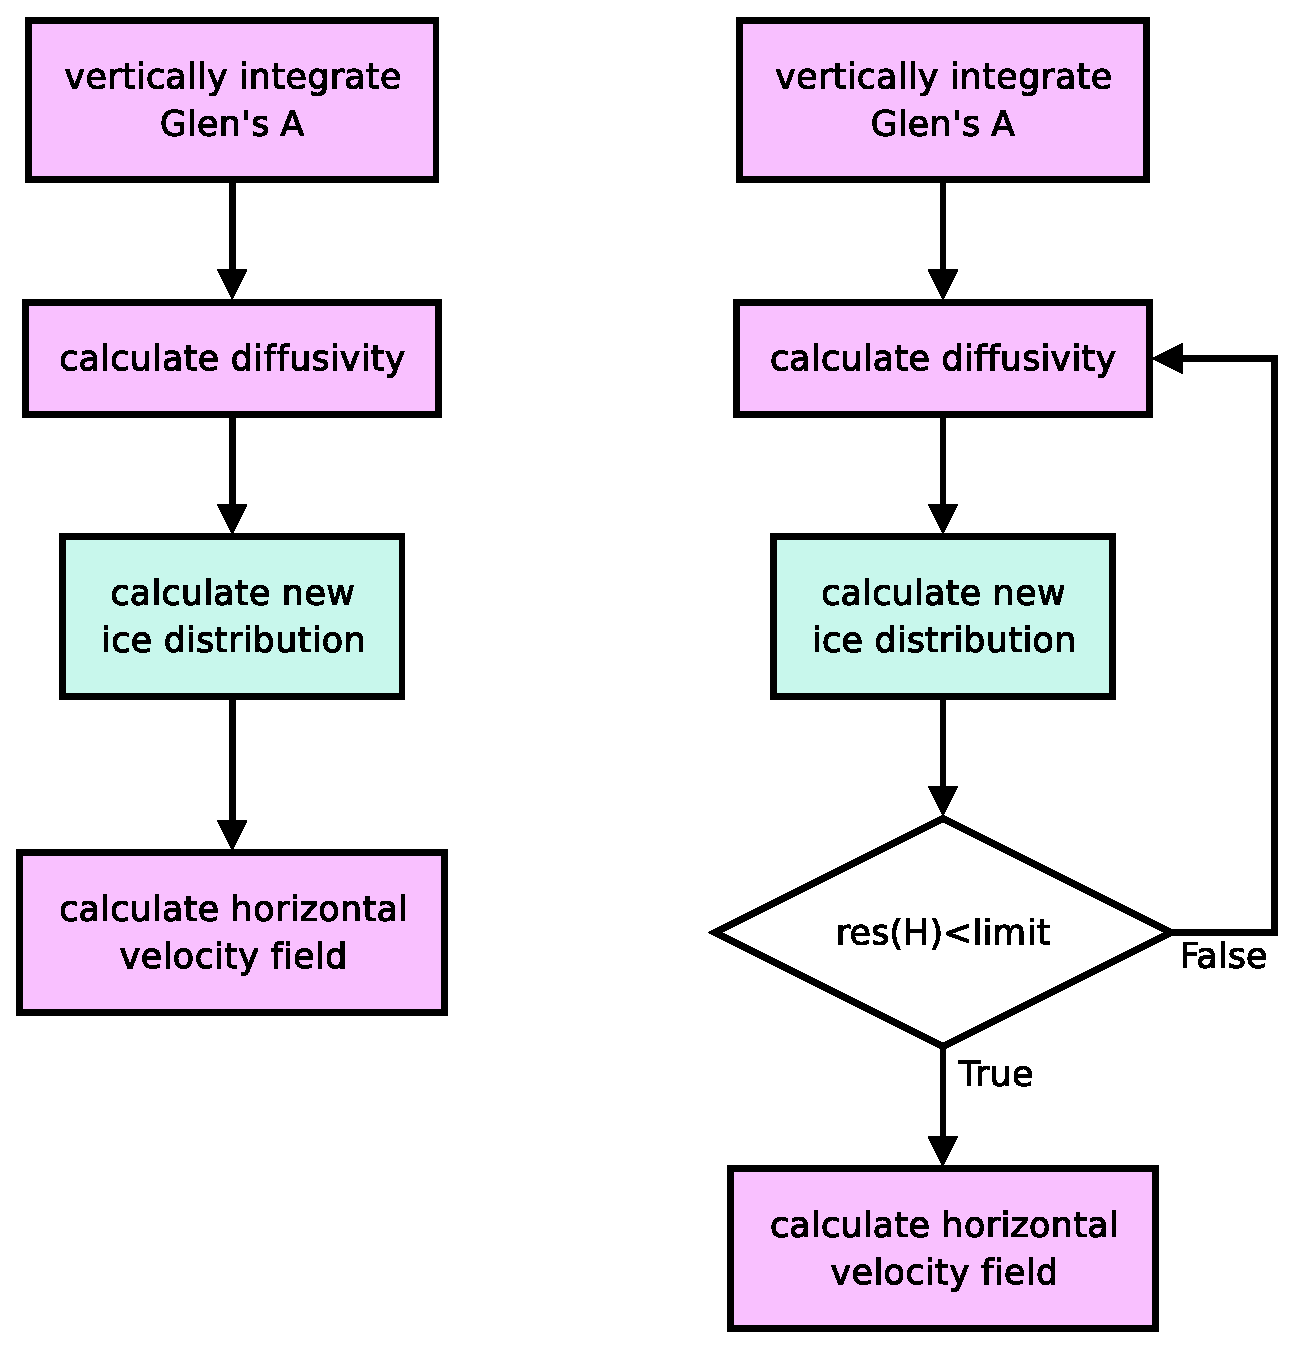
\epsfig{file=\dir/figs/thick_evo.eps,width=0.5\textwidth}
  \caption{Flow diagram showing how the linearised solver (on the left) and the non--linear solver work. The inner, linear iteration is contained within the box labeled ``calculate new ice distribution''.}
  \label{kin.fig.solvers}
\end{figure}

\subsection{Calculating Vertical Velocities}

\subsubsection{Grid Velocity}
The vertical grid moves as a consequence of using a $\sigma$--coordinate system. The grid velocity is
\begin{equation}
  \label{kin.eq.grid_velo}
  w^{\text{grid}}(\sigma)=\frac{\pd s}{\pd t}+\vec u\cdot\vec\nabla s-\sigma\left(\frac{\pd H}{\pd t}+\vec u\cdot\vec\nabla H\right)
\end{equation}
The numerical implementation of Equation \eqref{kin.eq.grid_velo} is straight--forward.

\subsubsection{Vertical Velocity}
The discretised version of the vertical velocity equation \eqref{kin.eq.vert_velo_scaled} is slightly more compilicated because the horizontal velocities are calculated on the $(r,s)$ grid. The vertical velocity at the ice base is $w_{i,j,N}=w^{\text{grid}}_{i,j,N}-b_{i,j}$, where $b_{i,j}$ is the basal melt rate. Integrating from the bottom, the vertical velocity is then
\begin{equation}
  \label{kin.eq.wvel_unc}
  \begin{split}
  w_{i,j,k}=-\sum_{\tilde{k}=N-1}^1\left\{\mathcal{H}_{i,j}\left(\frac{u^x_{i,j,k}+u^x_{i,j,k+1}}{2}+\frac{v^y_{i,j,k}+v^y_{i,j,k+1}}{2}\right)(\sigma_{k+1}-\sigma_k)\right. \\
     +(\tilde{u}_{i,j,k+1}-\tilde{u}_{i,j,k})  \left(\tilde{s}^x_{i,j}-\frac12(\sigma_{k+1}+\sigma_k)\tilde{H}^x_{i,j}\right)  \\
     \left.+(\tilde{v}_{i,j,k+1}-\tilde{v}_{i,j,k})  \left(\tilde{s}^y_{i,j}-\frac12(\sigma_{k+1}+\sigma_k)\tilde{H}^y_{i,j}\right)\right\} + w_{i,j,N}
  \end{split}
\end{equation}
with the weighted ice thickness
\begin{equation*}
  \begin{split}
  \mathcal{H}_{i,j}=\frac{4H_{i,j}+2(H_{i-1,j}+H_{i+1,j}+H_{i,j-1}+H_{i,j+1})}{16}\\
  +\frac{H_{i-1,j-1}+H_{i+1,j-1}+H_{i+1,j+1}+H_{i-1,j+1}}{16}    
  \end{split}
\end{equation*}

This scheme produces vertical velocities at the ice divide which are too small. The vertical velocities on the ice surface are given by the upper kinematic boundary condition, Equation \eqref{kin.eq.upper_bc}. Equation \eqref{kin.eq.wvel_unc} can be corrected with:
\begin{equation}
  \label{kin.eq.wvel_cor}
   w^\ast_{i,j,k}=w_{i,j,k}-(1-\sigma_k)(w_{i,j,k}-{w_s}_{i,j}),
\end{equation}
where ${w_s}_{i,j}$ is the vertical velocity at the ice surface given by \eqref{kin.eq.upper_bc}. Figure \ref{kin.fig.w_profile} shows the different vertical velocities at the ice surface.
\begin{figure}[htbp]
  \centering
  \includegraphics{\dir/gnu/w_profile.eps}
  \caption{Vertical ice surface velocities of the EISMINT-1 moving margin experiment.}
  \label{kin.fig.w_profile}
\end{figure}
The difference between the vertical velocities calculated by the model and the vertical velocities given by \eqref{kin.eq.upper_bc} at the ice margin are due to the fact that temperatures and velocities are only calculated when the ice is thicker than a certain threshold value which is not met at the ice margin.

Figure \ref{kin.fig.wt_sigma} shows vertical profiles of the vertical velocity at the ice divide and a point half--way between the divide and the domain margin. A corresponding temperature profile is also shown since the vertical velocity determines the vertical temperature advection (see Section \ref{temp.sec.vert_ad}).
\begin{figure}[htbp]
  \centering
  \includegraphics{\dir/gnu/wt_sigma.eps}
  \caption{Vertical velocity and temperature distribution for columns at the ice divide and a point half--way between the divide and the domain margin.}
  \label{kin.fig.wt_sigma}
\end{figure}
